%%%%%%%%%%%%%%%%%%%% chapter.tex (Chapter 6) %%%%%%%%%%%%%%%%%%%%%%%%%%%%%
% Chapter 6: Low-Power Architectures & Dark Silicon Dynamics
%%%%%%%%%%%%%%%%%%%%%%%%%%%%%%%%%%%%%%%%%%%%%%%%%%%%%%%%%%%%%%%%%%%%%%%%%

\chapter{Low-Power Architectures \& Dark Silicon Dynamics}
\label{ch:low_power}

\author{NoC-Lab Research Consortium}
\institute{NoC-Lab Research Consortium \at Shanghai Jiao Tong University \& International Collaborators, \email{research@network-on-chip.org}}

\maketitle

\abstract*{The demise of classical Dennard scaling has driven modern semiconductor manycores into the dark silicon era, where up to 80\% of the silicon floorplan must remain powered off or severely throttled under strict Thermal Design Power (TDP) constraints. While idle compute cores can be gated completely, on-chip interconnection routers must remain active to forward transit flits, making the network a primary power and thermal bottleneck. This chapter provides a comprehensive treatment of low-power NoC architectures. We formulate dynamic and static leakage power dynamics, model temperature-dependent sub-threshold leakage, and derive the breakeven idle time for power gating. We examine Dynamic Voltage and Frequency Scaling (DVFS) across Voltage-Frequency Islands (VFIs) and analyze the LAURA-NoC distributed rate adjustment architecture. Furthermore, we investigate ultrafine-grained run-time power gating across router virtual channels and crossbar multiplexers with lookahead early wake-up, analyze information-theoretic link code reordering (LPCR, IEEE TCAD 2025), and contrast buffered routers with bufferless deflection routing.}

\abstract{The demise of classical Dennard scaling has driven modern semiconductor manycores into the dark silicon era, where up to 80\% of the silicon floorplan must remain powered off or severely throttled under strict Thermal Design Power (TDP) constraints. While idle compute cores can be gated completely, on-chip interconnection routers must remain active to forward transit flits, making the network a primary power and thermal bottleneck. This chapter provides a comprehensive treatment of low-power NoC architectures. We formulate dynamic and static leakage power dynamics, model temperature-dependent sub-threshold leakage, and derive the breakeven idle time for power gating. We examine Dynamic Voltage and Frequency Scaling (DVFS) across Voltage-Frequency Islands (VFIs) and analyze the LAURA-NoC distributed rate adjustment architecture. Furthermore, we investigate ultrafine-grained run-time power gating across router virtual channels and crossbar multiplexers with lookahead early wake-up, analyze information-theoretic link code reordering (LPCR, IEEE TCAD 2025), and contrast buffered routers with bufferless deflection routing.}

\section{The Power Wall and the Dark Silicon Interconnect Bottleneck}
\label{sec:ch6_dark_silicon}
\index{Dark Silicon}
\index{Thermal Design Power (TDP)}
\index{Sub-Threshold Leakage}

At sub-7nm process nodes, the physical breakdown of classical Dennard scaling imposes an unyielding thermal dissipation ceiling ($\approx 100$--$150\text{ W/cm}^2$). Consequently, modern manycore chips face the \textbf{Dark Silicon Phenomenon}~\cite{Esmaeilzadeh2011}: between 50\% and 80\% of a chip's total transistor budget cannot be operated simultaneously at peak clock frequency without triggering thermal destruction.

While idle compute cores can be power-gated to zero power for milliseconds at a time, the \textbf{on-chip network cannot be casually turned off}. In multi-hop topologies (such as 2D Meshes), an intermediate router must remain awake to forward packets between active compute tiles. Routers sit active but idle for up to 90\% of total execution time~\cite{Matsutani2011}, dissipating substantial static leakage power.

\subsection{Dennard Breakdown and the Dark Silicon Scaling Model}
\label{subsec:ch6_dennard}
\index{Dennard Scaling}

To understand why power gating and voltage islands are mandatory in modern on-chip networks, one must examine the mathematical breakdown of classical Dennard scaling.

Under ideal Dennard scaling (formulated by Robert Dennard in 1974), all spatial geometric dimensions of a MOSFET scale down by a constant scaling factor $S > 1$ (where $S \approx \sqrt{2} \approx 1.4$ per technology generation):
\begin{equation}
L \longrightarrow \frac{L}{S}, \quad W \longrightarrow \frac{W}{S}, \quad t_{ox} \longrightarrow \frac{t_{ox}}{S}, \quad N_A \longrightarrow S \cdot N_A
\end{equation}
To maintain a constant electric field ($\mathcal{E} = V / t_{ox}$), the supply voltage $V_{dd}$ and threshold voltage $V_{th}$ were scaled simultaneously by $1/S$:
\begin{equation}
V_{dd} \longrightarrow \frac{V_{dd}}{S}, \quad V_{th} \longrightarrow \frac{V_{th}}{S}
\end{equation}
Consequently, gate capacitance scaled as $C = \epsilon A / t_{ox} \to C/S$, gate delay improved as $\tau = C V / I \to \tau / S$, allowing clock frequency to increase as $f_{clk} \to S \cdot f_{clk}$. The dynamic power per transistor evolved as:
\begin{equation}
P_{trans} = C \cdot V_{dd}^2 \cdot f_{clk} \longrightarrow \left(\frac{C}{S}\right) \left(\frac{V_{dd}}{S}\right)^2 (S \cdot f_{clk}) = \frac{P_{trans}}{S^2}
\label{eq:ch6_dennard_power}
\end{equation}
Because transistor density increased by $S^2$ per unit area, the total power density across the silicon die remained perfectly invariant:
\begin{equation}
\text{Power Density} = \frac{N_{trans} \cdot P_{trans}}{\text{Die Area}} \longrightarrow \frac{(S^2 \cdot N_{trans}) \cdot (P_{trans} / S^2)}{\text{Area}} = \text{Constant}
\end{equation}

Around 2005 (at the 90nm/65nm transition), Dennard scaling collapsed because \textbf{voltage scaling stalled}. The sub-threshold slope of a MOSFET is fundamentally constrained by Boltzmann thermodynamics:
\begin{equation}
S_S = \ln(10) \cdot \frac{k_B T}{q} \cdot \left(1 + \frac{C_d}{C_{ox}}\right) \ge 60\text{ mV/decade at } 300\text{ K}
\label{eq:ch6_subthreshold_slope}
\end{equation}
where $k_B$ is the Boltzmann constant, $T$ is absolute temperature, and $q$ is elementary charge. Because $S_S$ cannot be scaled below $60\text{ mV/decade}$ at room temperature, reducing $V_{th}$ causes off-state drain current $I_{off}$ to increase exponentially:
\begin{equation}
I_{off} = I_0 \cdot 10^{-V_{th} / S_S}
\label{eq:ch6_ioff}
\end{equation}
To prevent static leakage from overwhelming total chip power, designers had to clamp $V_{dd}$ to $\approx 0.75$--$0.95\text{ V}$.

With $V_{dd}$ fixed while transistor density continues to scale at $S^2$, chip power density escalates by $S^2$ each generation. Esmaeilzadeh et al.~\cite{Esmaeilzadeh2011} formulated the \textbf{Dark Silicon Utilization Fraction $U(S)$}:
\begin{equation}
U(S) = \frac{P_{TDP}}{P_{active}(S)} = \frac{P_{TDP}}{N_{trans}(S) \cdot C(S) \cdot V_{dd}^2(S) \cdot f_{clk}(S)} \approx \frac{1}{S^2} \left(\frac{V_{dd, 0}}{V_{dd}(S)}\right)^2 \left(\frac{f_0}{f_{clk}(S)}\right)
\label{eq:ch6_utilization}
\end{equation}
At advanced FinFET nodes (sub-5nm), $U(S) < 0.20$, proving that \textbf{over 80\% of the silicon floorplan must remain powered off or severely underclocked} at any given instant.

\subsection{Physical Power Breakdown in Nanoscale Routers}
Total interconnect power dissipation is decomposed into dynamic and static leakage components:
\begin{equation}
P_{total} = P_{dynamic} + P_{leakage}
\label{eq:ch6_ptotal}
\end{equation}

\textbf{Dynamic Power ($P_{dynamic}$)}: Consumed during capacitive charging and discharging across buffer cells, multiplexer trees, pipeline registers, and metal link wires:
\begin{equation}
P_{dynamic} = \alpha \cdot C_{eff} \cdot V_{dd}^2 \cdot f_{clk}
\label{eq:ch6_pdyn}
\end{equation}
where $\alpha$ is the switching activity factor, $C_{eff}$ is effective capacitance, $V_{dd}$ is supply voltage, and $f_{clk}$ is operating frequency.

\textbf{Static Leakage Power ($P_{leakage}$)}: Dominated by sub-threshold drain-source conduction $I_{sub}$ and gate oxide quantum tunneling:
\begin{equation}
I_{sub} = \mu_0 C_{ox} \frac{W}{L} (m - 1) V_T^2 \exp\left(\frac{V_{gs} - V_{th}}{m V_T}\right) \left(1 - \exp\left(-\frac{V_{ds}}{V_T}\right)\right)
\label{eq:ch6_leakage}
\end{equation}
Sub-threshold leakage scales exponentially with absolute temperature $T$ ($V_T = k_B T / q$). In sub-28nm geometries, static leakage constitutes between 40\% and 80\% of total router power dissipation.

\section{DVFS and Voltage-Frequency Islands (VFIs)}
\label{sec:ch6_dvfs}
\index{Dynamic Voltage and Frequency Scaling (DVFS)}
\index{Voltage-Frequency Islands (VFIs)}
\index{LAURA-NoC}
\index{Clock Domain Crossing (CDC)}

Dividing a large manycore into \textbf{Voltage-Frequency Islands (VFIs)} enables independent, dynamic adjustment of supply voltage and clock frequency across local network domains.

\begin{figure}[htbp]
\centering
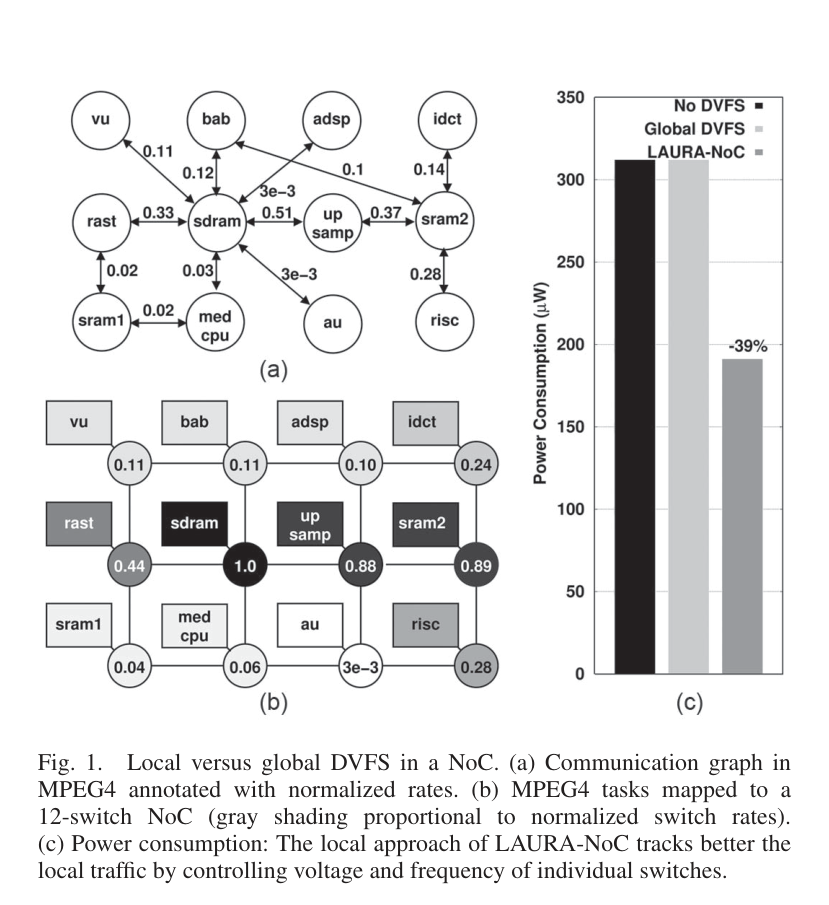
\includegraphics[width=0.75\textwidth]{chapters/ch06-low-power-dark-silicon/figures/yadav_fig01_laura_dvfs.png}
\caption{The LAURA-NoC distributed DVFS architecture: local hardware monitors input switch buffer occupancy in a feedback loop, dynamically adapting voltage and frequency without centralized controller overhead. [Reproduced from: M. K. Yadav, M. R. Casu, and M. Zamboni, ``LAURA-NoC: Local Automatic Rate Adjustment in Network-on-Chips With a Simple DVFS,'' \emph{IEEE Trans. Circuits Syst. II, Express Briefs}, Vol.~60, No.~10, pp.~647--651, October 2013, DOI: 10.1109/TCSII.2013.2278077. \copyright~2013 IEEE]}
\label{fig:ch6_laura}
\end{figure}

Yadav, Casu, and Zamboni~\cite{Yadav2013} developed \textbf{LAURA-NoC}, which eliminates global controller latency by measuring local switch buffer fullness to drive local voltage-frequency transitions. In 45nm CMOS, LAURA-NoC achieved \textbf{33\% average power savings} across realistic video processing workloads.

\subsection{Asynchronous Clock Domain Crossing (CDC) and Dual-Clock FIFOs}
When neighboring routers or tiles reside in distinct VFIs, signals must cross asynchronous clock domain boundaries. Direct sampling of asynchronous signals induces catastrophic \textbf{metastability}, where flip-flop internal nodes linger at an indeterminate voltage between 0 and 1, producing non-deterministic timing violations.

To guarantee robust inter-VFI communication, link interfaces employ \textbf{Dual-Clock Asynchronous FIFOs} with Gray-coded read and write pointers:
\begin{enumerate}
    \item \textbf{Gray-Code Pointer Synchronization}: The binary write pointer $B = (b_n, \dots, b_0)$ is converted to Gray code $G = (g_n, \dots, g_0)$ via $g_i = b_i \oplus b_{i+1}$. Gray codes ensure that \textbf{exactly one bit changes value per pointer increment}. Consequently, clock skew across the asynchronous boundary can at most cause the synchronizer to read the old pointer value or the new pointer value, but never an invalid intermediate state.
    \item \textbf{Two-Stage Synchronizer Reliability}: Dual-stage flip-flop synchronizers achieve an astronomical \textbf{Mean Time Between Failures (MTBF)}:
    \begin{equation}
    MTBF = \frac{\exp(t_{settle} / \tau_s)}{T_0 \cdot f_{dest} \cdot f_{src}}
    \label{eq:ch6_mtbf}
    \end{equation}
    where $\tau_s$ is the latch regeneration time constant, $T_0$ is the aperture parameter, $t_{settle}$ is the available settling time (one destination clock period minus setup time), $f_{src}$ is the transmitter clock frequency, and $f_{dest}$ is the receiver clock frequency.
    \item \textbf{Mixed-Clock Credit Loop Latency}: Flow control credits traversing the reverse path must also cross a two-stage synchronizer, introducing an unavoidable latency overhead of $2$--$3$ destination clock cycles into the credit return path. To sustain peak throughput without stalls, the asynchronous FIFO depth must satisfy:
    \begin{equation}
    \text{Depth}_{CDC} \ge 2 \cdot (RTT_{credit} + \text{Sync Delay}) = 2 \cdot (t_{link} + 2 \cdot T_{src} + 2 \cdot T_{dest})
    \label{eq:ch6_cdc_depth}
    \end{equation}
\end{enumerate}

\subsection{Feedback Control Theory for Autonomous VFI Frequency Scaling}
\label{subsec:ch6_pid_control}
\index{PID Controller}
\index{VFI Control Theory}

While centralized operating system governors can modulate tile frequencies at millisecond granularity, on-chip network packet bursts occur at nanosecond timescales ($10\text{--}100$ clock cycles). Autonomous VFIs deploy hardware-synthesized \textbf{Proportional-Integral-Derivative (PID) feedback controllers} embedded directly within router input controllers.

Let $q(t)$ denote the instantaneous flit occupancy of the input buffer, and let $Q_{\mathrm{target}}$ be the optimal setpoint (typically $30\%\text{--}50\%$ of maximum FIFO capacity to balance throughput against queuing latency). The error signal is:
\begin{equation}
e(t) = q(t) - Q_{\mathrm{target}}
\label{eq:ch6_error}
\end{equation}
The continuous rate of change of buffer fullness is governed by the mass balance equation:
\begin{equation}
\frac{d q(t)}{dt} = \lambda_{\mathrm{in}}(t) - \mu(f_{\mathrm{clk}}(t))
\label{eq:ch6_buffer_derivative}
\end{equation}
where $\mu(f_{\mathrm{clk}}) \approx \kappa_{\mu} \cdot f_{\mathrm{clk}}$ represents the crossbar flit forwarding rate.

In discrete hardware, the PID controller updates the clock frequency setpoint at sampling period $T_s$:
\begin{equation}
f_{\mathrm{clk}}[k+1] = f_{\mathrm{clk}}[k] + K_p \cdot e[k] + K_i \sum_{m=0}^k e[m] + K_d (e[k] - e[k-1])
\label{eq:ch6_pid_discrete}
\end{equation}
where $K_p, K_i, K_d$ are the proportional, integral, and derivative control gains.

\begin{svgraybox}
\textbf{Closed-Loop Stability \& Phase Margin}: By taking the $\mathcal{Z}$-transform of Eq.~(\ref{eq:ch6_pid_discrete}) combined with the buffer integrator plant $G(z) = \frac{T_s}{z - 1}$, the closed-loop characteristic equation is:
\begin{equation}
1 + D(z) G(z) = 0 \iff z^2 + \left( K_p T_s + K_i T_s + K_d - 2 \right) z + \left( 1 - K_p T_s - 2 K_d \right) = 0
\end{equation}
Applying Jury's stability criterion mandates that the loop gains satisfy $K_i T_s < 2$ and $K_d < \frac{1}{2} (1 - K_p T_s)$. To prevent destructive limit-cycle hunting under bursty traffic, controllers enforce a \textbf{Bode phase margin} of $\phi_m \ge 60^\circ$ and implement deadband hysteresis around $Q_{\mathrm{target}}$.
\end{svgraybox}

Furthermore, physical hardware actuators impose strict transient slew rate constraints:
\begin{itemize}
    \item \textbf{Phase-Locked Loop (PLL) Relock Delay}: Frequency changes require $t_{\mathrm{relock}} \approx 20\text{--}50\,\mathrm{ns}$ for voltage-controlled oscillators to stabilize without clock glitching.
    \item \textbf{Integrated Voltage Regulators (IVR)}: On-chip buck converters and switched-capacitor DC-DC converters are limited by an inductive slew rate ceiling ($dV/dt \le 10\text{--}25\,\mathrm{mV/\mu s}$), dictating that frequency steps must lead voltage drops but lag voltage rises to prevent timing failure.
\end{itemize}

\subsection{Near-Threshold Computing (NTC) Interconnects \& Razor Timing Speculation}
\label{subsec:ch6_ntc}
\index{Near-Threshold Computing (NTC)}
\index{Razor Flip-Flops}

The most aggressive low-power regime is \textbf{Near-Threshold Computing (NTC)}, where supply voltage is scaled down to just above the transistor threshold ($V_{dd} \approx V_{th} + 100\text{--}150\,\mathrm{mV} \approx 0.40\text{--}0.50\,\mathrm{V}$). Because dynamic energy scales quadratically ($E \propto C V_{dd}^2$), NTC slashes interconnect energy by \textbf{$5\times$ to $10\times$}.

However, NTC faces the \textbf{Variability Wall}. Under the alpha-power law model, CMOS gate delay $t_d$ is:
\begin{equation}
t_d = \frac{C_{\mathrm{load}} \cdot V_{dd}}{\mu C_{ox} \frac{W}{L} (V_{dd} - V_{th})^\alpha}
\label{eq:ch6_alpha_power}
\end{equation}
with velocity saturation index $\alpha \approx 1.3\text{--}1.5$. Differentiating Eq.~(\ref{eq:ch6_alpha_power}) with respect to $V_{dd}$ reveals the normalized delay sensitivity:
\begin{equation}
\mathcal{S}_{V_{dd}}^{t_d} = \frac{\partial t_d / t_d}{\partial V_{dd} / V_{dd}} = 1 - \frac{\alpha V_{dd}}{V_{dd} - V_{th}}
\label{eq:ch6_ntc_sensitivity}
\end{equation}
At nominal $V_{dd} = 0.90\,\mathrm{V}$ ($V_{th} = 0.35\,\mathrm{V}$), $|\mathcal{S}| \approx 1.1$. But in NTC ($V_{dd} = 0.45\,\mathrm{V}$), $V_{dd} - V_{th} = 0.10\,\mathrm{V}$, causing sensitivity to escalate to $|\mathcal{S}| \approx 5.8$! A mere $5\%$ power grid IR-drop ($22\,\mathrm{mV}$) triggers a catastrophic \textbf{$30\%$ gate delay surge}, causing widespread setup-time violations.

To operate safely in NTC without exorbitant worst-case guardbands, routers employ \textbf{Razor Timing Speculation}:
\begin{enumerate}
    \item Each critical flip-flop is paired with a delayed \textbf{Shadow Latch} clocked by a delayed clock phase ($\Delta t_{\mathrm{margin}}$).
    \item If a slow path violates setup time at the main flip-flop, the shadow latch captures the correct late-arriving data.
    \item An XOR comparator flags the timing error, asserts a pipeline squash pulse, replays the cycle from the shadow latch, and dynamically nudges the local VFI voltage regulator higher.
\end{enumerate}

\section{Ultrafine-Grained Run-Time Power Gating}
\label{sec:ch6_power_gating}
\index{Power Gating}
\index{Sleep Transistors}
\index{Breakeven Time}

Power gating completely disconnects inactive logic blocks from the power rails using high-threshold sleep transistors (power switches).

\begin{figure}[htbp]
\centering
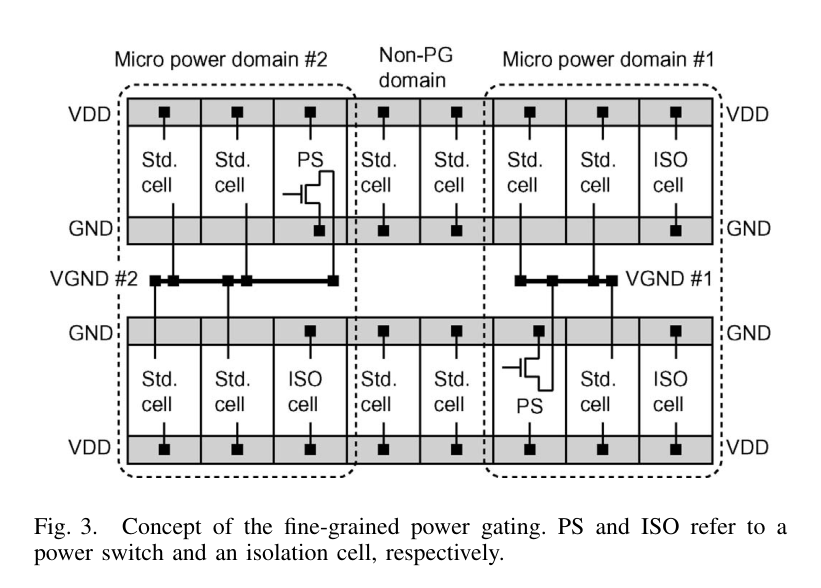
\includegraphics[width=0.75\textwidth]{chapters/ch06-low-power-dark-silicon/figures/matsutani_fig03_power_switch.png}
\caption{Concept of fine-grained run-time power gating. (a) Active mode: power switch (PS) is closed, virtual VDD rail is at nominal potential. (b) Sleep mode: PS opens, cutting leakage; isolation cells (ISO) clamp boundary outputs to prevent downstream crowbar currents. [Reproduced from: H. Matsutani et al., ``Performance, Area, and Power Evaluations of Ultrafine-Grained Run-Time Power-Gating Routers for CMPs,'' \emph{IEEE Trans. Comput.-Aided Design Integr. Circuits Syst.}, Vol.~30, No.~4, pp.~520--533, April 2011, DOI: 10.1109/TCAD.2010.2097310. \copyright~2011 IEEE]}
\label{fig:ch6_power_switch}
\end{figure}

\begin{figure}[htbp]
\centering
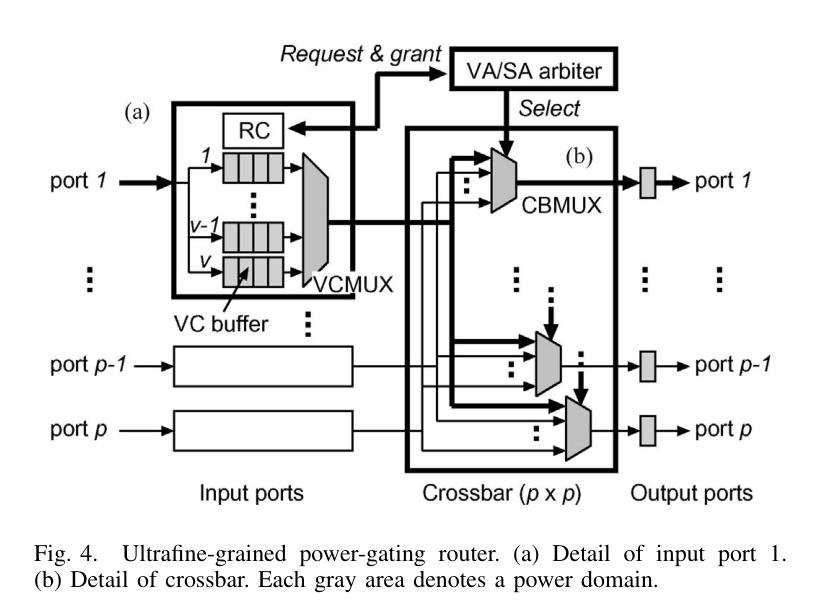
\includegraphics[width=0.75\textwidth]{chapters/ch06-low-power-dark-silicon/figures/matsutani_fig04_power_gated_router.png}
\caption{Ultrafine-grained power-gating router microarchitecture: (a) detail of input port virtual channel buffers and multiplexers; (b) detail of crossbar multiplexers. Each shaded partition represents an independently gated domain. [Reproduced from: H. Matsutani et al., ``Performance, Area, and Power Evaluations of Ultrafine-Grained Run-Time Power-Gating Routers for CMPs,'' \emph{IEEE Trans. Comput.-Aided Design Integr. Circuits Syst.}, Vol.~30, No.~4, pp.~520--533, April 2011, DOI: 10.1109/TCAD.2010.2097310. \copyright~2011 IEEE]}
\label{fig:ch6_matsutani_router}
\end{figure}

Matsutani et al.~\cite{Matsutani2011} proved that ultrafine-grained partitioning of router buffers and crossbar multiplexer slices eliminates \textbf{over 70\% of static leakage}.

\subsection{Sleep Transistor Sizing and In-Rush Damping}
\label{subsec:ch6_sleep_sizing}
Sleep transistors are deployed either as \textbf{Header switches} (PMOS transistors inserted between true $V_{dd}$ and virtual $V_{ddv}$) or \textbf{Footer switches} (NMOS transistors inserted between virtual ground $V_{ssv}$ and true ground). While NMOS footers provide higher electron mobility ($\mu_n \approx 2\text{--}3 \times \mu_p$) and smaller silicon area, PMOS headers are vastly preferred in NoCs because modulating ground potential disrupts substrate body bias and induces substrate noise coupling across adjacent analog/memory IPs.

The width of the sleep transistor $W_{sleep}$ is strictly governed by the peak active current $I_{peak}$ and the maximum allowable virtual rail IR-drop budget $\Delta V_{drop}$ (typically $\le 1.5\%$ of $V_{dd}$):
\begin{equation}
W_{sleep} = \frac{I_{peak}}{\mu_p C_{ox} \left(\frac{W}{L}\right)_{min} (V_{dd} - |V_{th, p}|) \cdot \Delta V_{drop}}
\label{eq:ch6_sleep_width}
\end{equation}

When awakening a sleeping router partition, abrupt gating causes a massive surge of \textbf{in-rush current} to charge the virtual rail capacitance $C_{virtual}$. This sudden current transient induces severe inductive supply bounce across package bond wires:
\begin{equation}
\Delta V_{bounce} = L_{pkg} \frac{d i_{rush}}{dt} + R_{pkg} \cdot i_{rush}
\label{eq:ch6_ground_bounce}
\end{equation}
Excessive $\Delta V_{bounce}$ can inadvertently flip state bits in adjacent active SRAM buffers. To mitigate this hazard, routers deploy \textbf{Two-Stage Sleep Switches}:
\begin{itemize}
    \item \textbf{Stage 1 (Weak Pre-Charge)}: A small, high-resistance sleep transistor turns on first, limiting $d i / dt$ while charging $V_{ddv}$ smoothly to $\approx 80\%$ of nominal voltage.
    \item \textbf{Stage 2 (Full Rail Clamping)}: The massive low-resistance main sleep transistor closes, clamping $V_{ddv}$ to full supply with minimal inductive ringing.
\end{itemize}

\subsection{Breakeven Idle Time Formulation}
Transitioning into and out of sleep mode consumes energy charging the virtual rail capacitance ($C_{virtual}$):
\begin{equation}
E_{overhead} \approx C_{virtual} \cdot V_{dd}^2
\label{eq:ch6_eoverhead}
\end{equation}
The minimum inactive duration required to achieve net energy savings is the \textbf{Breakeven Idle Time ($\tau_{breakeven}$)}:
\begin{equation}
\tau_{breakeven} = \frac{E_{overhead}}{P_{leak\_active}} = \frac{C_{virtual} \cdot V_{dd}}{I_{leak\_active}}
\label{eq:ch6_breakeven}
\end{equation}
In modern technologies, $\tau_{breakeven}$ spans only 2 to 6 clock cycles, making run-time power gating highly energy-positive.

\subsection{Lookahead Early Wake-Up}
To eliminate the 2-to-4 cycle wakeup latency penalty, upstream routers transmit an early wakeup pulse across dedicated physical wires one hop ahead of flit departure, charging the downstream virtual rail concurrently with upstream crossbar traversal.

\section{Low-Power Link Encoding: The LPCR Framework}
\label{sec:ch6_lpcr}
\index{Link Encoding}
\index{LPCR Framework}

Long inter-router metal links exhibit severe inter-wire coupling capacitance ($C_{coupling} \approx 3\text{--}5 \times C_{ground}$). Opposite-direction signal transitions ($01 \to 10$) trigger Miller effect capacitance doubling.

\begin{figure}[htbp]
\centering
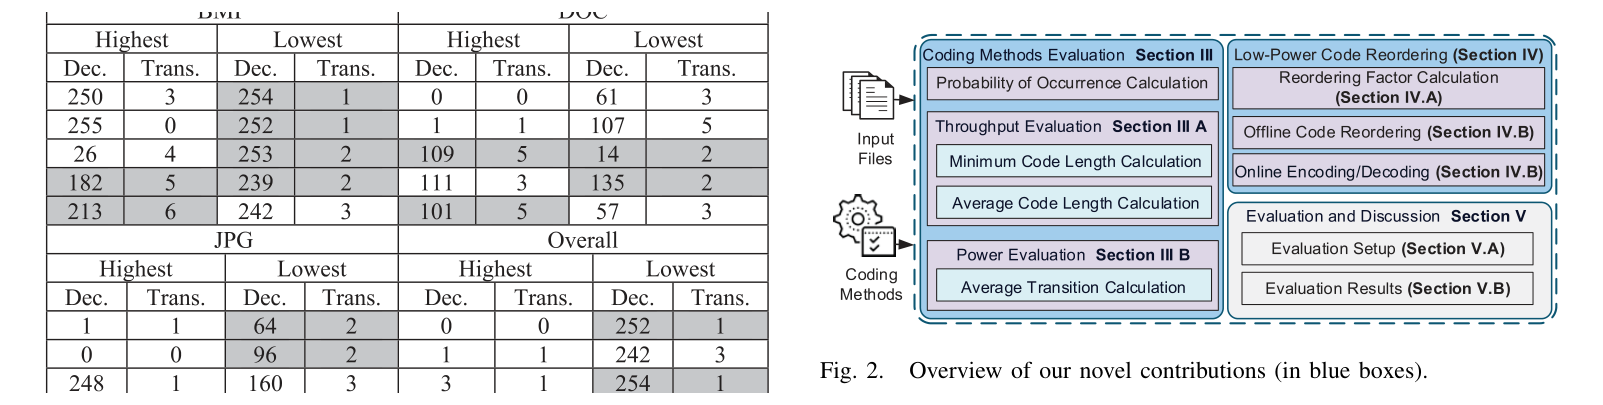
\includegraphics[width=0.85\textwidth]{chapters/ch06-low-power-dark-silicon/figures/adelkhani_fig02_lpcr_arch.png}
\caption{The LPCR (Low-Power Code Reordering) framework: information-theoretic analysis of data streams reorders binary codewords to minimize bit transitions across global serial links. [Reproduced from: M. Adelkhani et al., ``LPCR: Information-Theory-Based Low-Power Code Reordering for Serial Links in Network-on-Chip,'' \emph{IEEE Trans. Comput.-Aided Design Integr. Circuits Syst.}, Vol.~44, No.~11, pp.~4155--4168, November 2025, DOI: 10.1109/TCAD.2025.3411245. \copyright~2025 IEEE]}
\label{fig:ch6_lpcr}
\end{figure}

Adelkhani et al.~\cite{Adelkhani2025} developed \textbf{LPCR}, mapping high-frequency data symbols onto minimum-transition binary codewords and slashing link dynamic power by up to 35\% without throughput degradation.

\section{Bufferless Deflection Routing}
\label{sec:ch6_bufferless}
\index{Bufferless Routing}
\index{Deflection Routing}
\index{BLESS}
\index{CHIPPER}

Moscibroda and Mutlu~\cite{Moscibroda2009} proposed an extreme low-power alternative: \textbf{eliminating router input FIFO buffers entirely} via bufferless deflection routing (such as BLESS and CHIPPER).

\subsection{Microarchitectural Mechanics and Flit Arbitration}
In a bufferless router, flits never stall in place awaiting available downstream buffers. Instead, every flit arriving at an input port in cycle $t$ \textbf{must exit through an output port in cycle $t+1$}:
\begin{enumerate}
    \item \textbf{Port Contention and Deflection}: When multiple incoming flits request the same output port, the arbiter grants the port to the highest-priority flit. The losing flit is not stalled; rather, it is \textbf{deflected} onto an alternative, non-optimal output port (hot-potato routing).
    \item \textbf{Livelock Freedom Proof}: To prevent deflected flits from wandering endlessly across the network without arriving at their destination, BLESS enforces an \textbf{Oldest-First Priority Policy}:
    \begin{equation}
    \text{Priority}(F_i) > \text{Priority}(F_j) \iff \text{Age}(F_i) > \text{Age}(F_j)
    \label{eq:ch6_bless_priority}
    \end{equation}
    Because every flit's age increments monotonically every clock cycle, the globally oldest flit in the fabric is guaranteed to win every port arbitration. It routes strictly along minimal paths without deflection until reaching its destination. Once it exits, the next oldest flit acquires peak priority. By mathematical induction, \textbf{livelock is provably impossible}.
\end{enumerate}

\subsection{The Energy Crossover Threshold}
While bufferless deflection routing completely eliminates 60\% to 75\% of router silicon area and removes all buffer static leakage power, it incurs significant trade-offs:
\begin{itemize}
    \item \textbf{Reassembly Buffer Overhead}: Due to deflections, flits belonging to the same packet arrive out of order at the destination Network Interface (NI). The NI must maintain dedicated reassembly buffers sized proportional to the maximum latency skew:
    \begin{equation}
    \text{Buffer}_{reassembly} \ge B_W \times \Delta t_{skew}
    \end{equation}
    \item \textbf{Dynamic Link Energy Crossover}: Every deflected hop causes an extra physical wire traversal, consuming dynamic link power $\alpha C_{link} V_{dd}^2$. At low injection loads ($\lambda < 0.15\text{ flits/node/cycle}$), deflections are rare, and bufferless networks achieve up to 40\% total energy savings. However, when injection exceeds the \textbf{crossover rate ($\lambda \ge 0.20$)}, deflection cascading causes dynamic link power to exceed the static buffer leakage savings, rendering bufferless architectures inefficient under high load.
\end{itemize}

\section{Quantitative Evaluation Matrix}
\label{sec:ch6_matrix}

Table~\ref{tab:ch6_power_comparison} summarizes the trade-offs of low-power interconnect methodologies across an $8 \times 8$ mesh fabric.

\begin{table}[htbp]
\centering
\caption{Quantitative Comparison of Low-Power Interconnect Architecture Paradigms}
\label{tab:ch6_power_comparison}
\begin{tabular}{lcccc}
\toprule
\textbf{Architecture} & \textbf{Dynamic Power} & \textbf{Leakage Power} & \textbf{Area Overhead} & \textbf{Latency Cost} \\
\midrule
Baseline (Fixed 0.9V/1.2GHz) & Baseline & Baseline & Baseline & 0 cycles \\
Distributed DVFS (LAURA-NoC) & -33\% to -45\% & -20\% & +4\% & 0--1 cycle \\
Ultrafine Power Gating & Baseline & -70\% to -95\% & +8\% & 0 (Lookahead) \\
Co-Design (DVFS + PG) & -40\% & -85\% & +12\% & 1 cycle \\
Link Reordering (LPCR) & -25\% (Links) & Baseline & +1.5\% & 0 cycles \\
Bufferless Deflection & +20\% (Links) & -75\% & -60\% (No FIFO) & +2--6 hops \\
\bottomrule
\end{tabular}
\end{table}

\section{Interactive Lab \& Hands-on Challenges}
\label{sec:ch6_interactive}

Explore the interactive power and energy visualizers on the \textbf{NoC Learning Hub} (\url{https://network-on-chip.github.io/learning/}):
\begin{itemize}
    \item \textbf{Volt Vortex: Dark Silicon Power} (\url{https://network-on-chip.github.io/learning/interactive/power/}): Balance active core voltage/frequency islands against router power-gating breakeven thresholds.
    \item \textbf{QoS Gladiator: Traffic Arbiter} (\url{https://network-on-chip.github.io/learning/interactive/qos/}): Schedule mixed-criticality traffic flows while managing dynamic voltage-frequency scaling margins.
\end{itemize}

\section{Exercises and Review Questions}
\label{sec:ch6_exercises}

\begin{enumerate}
    \item \textbf{Breakeven Time Calculation}: A router buffer in 28nm FinFET has $C_{virtual} = 3.2\text{ pF}$, $V_{dd} = 0.85\text{ V}$, and $I_{leak} = 8.5\text{ mA}$ at $75^\circ\text{C}$. Calculate $E_{overhead}$ and $\tau_{breakeven}$. At $1.5\text{ GHz}$, how many idle cycles justify sleeping?
    \item \textbf{DVFS Power Scaling}: If supply voltage is reduced from $1.0\text{ V}$ to $0.75\text{ V}$ and frequency scales from $1.5\text{ GHz}$ to $1.0\text{ GHz}$, calculate the percentage reduction in dynamic power.
    \item \textbf{Lookahead Wakeup Hazards}: Describe the circuit consequences if a flit arrives at a power-gated buffer whose virtual power rail has only reached 50\% of nominal voltage.
\end{enumerate}

\section{References \& Further Reading}
\label{sec:ch6_references}

\begin{enumerate}
    \item \textbf{[Esmaeilzadeh2011]} H.~Esmaeilzadeh, E.~Blem, R.~St.~Amant, K.~Sankaralingam, and D.~Burger, ``Dark Silicon and the End of Multicore Scaling,'' in \emph{Proceedings of the 38th Annual International Symposium on Computer Architecture (ISCA)}, 2011, pp.~365--376. \url{https://doi.org/10.1145/2000064.2000108}
    \item \textbf{[Matsutani2011]} H.~Matsutani, M.~Koibuchi, D.~Ikebuchi, K.~Usami, H.~Nakamura, and H.~Amano, ``Performance, Area, and Power Evaluations of Ultrafine-Grained Run-Time Power-Gating Routers for CMPs,'' \emph{IEEE Transactions on Computer-Aided Design of Integrated Circuits and Systems}, vol.~30, no.~4, pp.~520--533, 2011. \url{https://doi.org/10.1109/TCAD.2010.2097310}
    \item \textbf{[Yadav2013]} M.~K.~Yadav, M.~R.~Casu, and M.~Zamboni, ``LAURA-NoC: Local Automatic Rate Adjustment in Network-on-Chips With a Simple DVFS,'' \emph{IEEE Transactions on Circuits and Systems--II: Express Briefs}, vol.~60, no.~10, pp.~647--651, 2013. \url{https://doi.org/10.1109/TCSII.2013.2278077}
    \item \textbf{[Adelkhani2025]} M.~Adelkhani, A.~Suvizi, F.~Arzaghi, S.~Zamani, M.~Salehi, and M.~Shafique, ``LPCR: Information-Theory-Based Low-Power Code Reordering for Serial Links in Network-on-Chip,'' \emph{IEEE Transactions on Computer-Aided Design of Integrated Circuits and Systems}, vol.~44, no.~11, pp.~4155--4168, 2025. \url{https://doi.org/10.1109/TCAD.2025.3411245}
    \item \textbf{[Moscibroda2009]} T.~Moscibroda and O.~Mutlu, ``A Case for Bufferless Routing in On-Chip Networks,'' in \emph{Proceedings of the 36th Annual International Symposium on Computer Architecture (ISCA)}, 2009, pp.~196--207. \url{https://doi.org/10.1145/1555754.1555780}
    \item \textbf{[Stan1995]} M.~R.~Stan and W.~P.~Burleson, ``Bus-Invert Coding for Low-Power I/O,'' \emph{IEEE Transactions on Very Large Scale Integration (VLSI) Systems}, vol.~3, no.~1, pp.~49--58, 1995. \url{https://doi.org/10.1109/92.365453}
\end{enumerate}
